\documentclass[a4paper, twocolumn]{article}
\usepackage[utf8]{inputenc}
\usepackage{amsmath}
\usepackage{tikz}
\usepackage{pgfplots}
\usepackage{mathtools}
\usepackage{setspace}
\usepackage{graphicx}
\usepackage{amssymb}
%\usepackage[nobottomtitles]{titlesec}
\setlength{\columnsep}{1.5cm}
\graphicspath{{C:/Users/krist/docs/Documents/Fizike/shenime/}}
\DeclarePairedDelimiter\abs{\lvert}{\rvert}
% \setlength{\extrarowheight}{2pt}
\pgfplotsset{width=7cm,compat=1.9}
\renewcommand{\arraystretch}{2.2}
\tolerance=1
\emergencystretch=\maxdimen
\hyphenpenalty=10000
\hbadness=10000
\clubpenalty = 10000
\renewcommand*\contentsname{Përmbajtja.}
\title{Permbledhje}
\author{Kristian Blido}
\date{03, 06 2021}
\begin{document}
\tableofcontents
\maketitle
% \addtocounter{section}{8}
\section{Kinematika}
\subsection{Shpejtesia Mesatare}
\[v=\frac{\Delta l}{\Delta t}\]
\subsection{Levizja me nxitim}
\begin{eqnarray*}
a & =&\frac{\Delta v}{\Delta t}\\
v & =& v_0 + a \cdot t\\
v^2 & =& v_{0}^{2}+2\cdot a \cdot l \\
l & =& v_{avg} \cdot t_{total} = \frac{v + v_0}{2} \cdot t \\
l & =& l_0 + v_0 \cdot t + \frac{a\cdot t^2}{2}
\end{eqnarray*}
\subsection{Levizja 2 permasore}
\begin{eqnarray*}
	v_x &=& v \cdot \cos\theta \\
	v_y &=& v \cdot \sin\theta \\
	t_{ajer} &=& \frac{2 \cdot v \cdot \sin \theta }{g}\\
	l_{max} &=& v_x \cdot \Delta t = \frac{v^2 \cdot \sin 2\theta}{g} \\
	h_{max} &=& \frac{v^2 \sin^2 \theta}{2\cdot g}\\
\end{eqnarray*}
\subsection{Levizja rrethore}
\[
\begin{array}{c c c c c c c}
	\theta &=& \theta_0 + \omega \cdot \Delta t &&&&\\
	\omega &=& \frac{\Delta \theta}{\Delta t} &=& 2\cdot \pi \cdot f&&\\
	v &=& r \cdot \omega&&&&\\
	a &=& r \cdot \omega^2 &=& \frac{v^2}{r}&&\\
	\vec{F} &=& m\cdot a &=& m\cdot \omega^2\cdot r &=& \frac{m \cdot v^2}{r}\\
\end{array}
\]
\section{Dinamika}
\[\sum  \mid \vec{F}  \mid = m \cdot a\]
\subsection{Terheqja Gravitacionale}
\begin{eqnarray*}
	g&=& \frac{\vec{G}}{m} \\
	\vec{G}&=&\gamma \cdot\frac{m_1 \cdot m_2}{r^2}\\
\end{eqnarray*}
\subsection{Pesha}
Forca qe vepron nga trupi tek mbeshtetsja ku eshte vendosur ose mbi fijen e varur.
\[ P = m \cdot \left( g-a \right)  \]
Nxitimi me kah lart $\to$ poshte e ben nxitimin rezultant me te vogel se ai fillestar $\left( g \right)$ dhe anasjelltas.
\subsection{Momenti}
\[
	M=\vec{F} \cdot d
\]
\subsection{Impulsi}
\[
	\vec{p} = m \cdot \vec{v}
\]
\[
	\Delta \vec{p} = \vec{F} \cdot  \Delta t
\]
\subsubsection{Ruajtja e Impulsit}
\[
	m_1 \cdot  v_1 + m_2 \cdot v_2 = m_1\cdot v_{1}'+ m_2\cdot v_{2}'
\]
\subsection{Susta}
$k$ : koeficienti i sustes  $\frac{N}{m}$
\[
	\vec{F} = - k \cdot x
\]
\begin{gather*}
	\omega = \sqrt{\frac{k}{m}} \\
	f = \frac{\omega}{2\cdot \pi} = \frac{\sqrt{\frac{k}{m}}}{2 \cdot \pi} \\
	T = 2 \cdot \pi \cdot \sqrt{\frac{m}{k}}
\end{gather*}
\subsubsection{Lidhja e sustave}
\paragraph{Lidhja ne seri}
\[
\frac{1}{k_r}= \frac{1}{k_1}+\frac{1}{k_2}
\]
\paragraph{Lidhja ne paralel}
\[
k_r = k_1+k_2
\]
\subsection{Lavjerresi}
\begin{gather*}
	\omega = \sqrt{\frac{g}{l}} \\
	f = \frac{1}{2\cdot \pi} \cdot  \sqrt{\frac{g}{l}} 
\end{gather*}
\section{Puna, Energjia, Fuqia}
\subsection{Puna}
\[
A = \Delta E
\]
\[
	A = \vec{F} \cdot \vec{x} =   F   \cdot  x  \cdot \cos \theta
\]
\subsection{Energjia}
\subsubsection{Mekanike}
\[
E_m=E_k + E_p
\]
\subsubsection{Kinetike}
\[
E_k = \frac{m\cdot v^2}{2}
\]
\subsubsection{Potenciale e lartesise}
\[
E_p = m\cdot g\cdot h
\]
\subsubsection{Potenciale elastike}
\[
E_{p_{elastike}} = \frac{k\cdot \Delta x^2}{2}
\]
\subsection{Fuqia}
 \[
	 P=\frac{A}{\Delta t}=\vec{F}\cdot \vec{v}=F\cdot v\cdot \cos\theta
\]
\section{Lenda dhe Materialet}
\subsection{Dendeisa}
\[
\rho = \frac{m}{v}=d
\]
\subsection{Shtypja}
\[
P=\frac{F}{S}
\]
\subsubsection{Shtypja brenda lengut}
\[
P=\rho\cdot g\cdot h
\]
\subsection{Sforcimi}
\[
	\sigma=\frac{F}{S}
\]
\subsection{Shformimi}
\[
\epsilon=\frac{x}{L}
\]
\subsection{Moduli i Young-ut}
\[
E=\frac{\sigma}{\epsilon}
\]
\section{Fizika Termike}
\subsection{Ndryshimi i Gjendjes dhe Energjise}
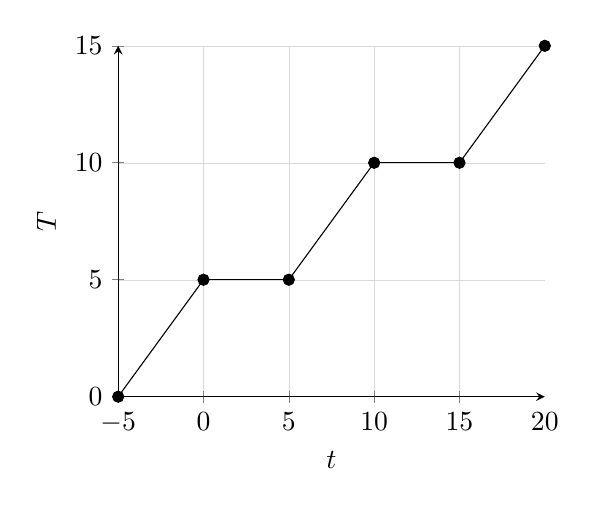
\begin{tikzpicture}
	\begin{axis}[
		axis lines = left,
    		xlabel = $t$,
    		ylabel = {$T$},
		grid=both,
		grid style={line width=.1pt, draw=gray!30},
		xtick={-5, 0, 5, 10, 15, 20}
		%minor tick num=5
		]
%Below the red parabola is defined
\addplot [
    domain=-5:0,
    samples=100,
    color=black,
]
{x+5};
\addplot [
    domain=0:5,
    samples=100,
    color=black,
]
{5};
\addplot [
    domain=5:10,
    samples=100,
    color=black,
]
{x};
\addplot [
    domain=10:15,
    samples=100,
    color=black,
]
{10};
\addplot [
    domain=15:20,
    samples=100,
    color=black,
]
{x-5};
	\addplot[mark=*] coordinates {(-5, 0)};
	\addplot[mark=*] coordinates {(0, 5)};
	\addplot[mark=*] coordinates {(5, 5)};
	\addplot[mark=*] coordinates {(10, 10)};
	\addplot[mark=*] coordinates {(15, 10)};
	\addplot[mark=*] coordinates {(20, 15)};
\end{axis}
\end{tikzpicture}
$$
	\begin{array}{r c l l}
	]-5, 0[ & \to&\textrm{Ngrohje}& Q=c\cdot m \cdot \Delta T \\
	]0, 5[ &\to& \textrm{Shkrirje}& Q=\lambda \cdot m \\
	]5, 10[ &\to& \textrm{Ngrohje}& Q=c\cdot m \cdot \Delta T  \\
	]10, 15[ &\to& \textrm{Avullim}& Q=q \cdot m\\
	]15, 20[ &\to& \textrm{Ngrohje}& Q=c\cdot m \cdot \Delta T \\
\end{array}
$$
\section{Gazet Ideale}
\[
	n=\frac{m}{M}=\frac{N}{N_{A}}
\]
\[
	T(K)=T(^{\circ}C)+273.15
\]
\subsection{Ligji i gazeve}
\begin{align*}
	P\cdot V &= N\cdot k_{b}\cdot T\\
	P\cdot V &= n\cdot (N_{A}\cdot k_{B})\cdot T\\
	P\cdot V &= n\cdot R\cdot T\\
	P\cdot M &= d\cdot R\cdot T
\end{align*}
\subsection{Energjia e Brendshme}
\[
U = \left\{
\begin{array}{l l l}
		\frac{3}{2}\cdot R\cdot T\cdot n, &1&\text{atom} \\
		\frac{5}{2}\cdot R\cdot T\cdot n, &2&\text{atome}\\
		3\cdot R\cdot T\cdot n, &3+&\text{atome}\\
\end{array}
\right.
\]
\[\begin{array}{ccccc}
	R&=&N_{A}&\cdot &k_{B}\\
	 &=&6.02\cdot 10^{23} \frac{}{mol} &\cdot & 1.38 \cdot \frac{m^2 kg}{10^{23}\cdot s^{2}\cdot K^{1}}   \\
	 &=&8.31 \frac{m^2\cdot kg}{s^{2}\cdot K\cdot mol}\\
	 &=&8.31 \frac{J}{mol\cdot K}
\end{array}
\]
\subsection{Energjia Kinetike}
\begin{eqnarray*}
	P &=& \frac{1}{3} \cdot  \frac{N}{V} \cdot m \cdot <v^2>\\
	  \\
	P &=& \frac{2}{3} \cdot \frac{N}{V} \cdot <\epsilon_{k}>\\
	  \\
	 \hline \\
	\\
	< \epsilon_{k}> &=& \frac{3}{2}\cdot k_{B}\cdot T\\
\end{eqnarray*}
\subsection{Puna e gazeve}
\[
A=P\cdot \Delta V
\]
\subsection{Parimi i pare i Termodinamikes}
\[
Q=\Delta U + A
\]
"Sasia e nxehtesise qe merr nje sistem shkon pjeserisht per ndryshimin e energjise se brendshme dhe pjeserisht per kryerjen e punes"
\subsection{Izoproceset}
\begingroup
\subsubsection{Ciklik}
\begin{itemize}
	\item 2 rruge Termodinamike
	\item Sisteme \emph{Quasi-Statike}
\end{itemize}
\[
\begin{Bmatrix}
T_{1}&=& T_{2} \\
\Delta U &=& 0 \\
Q &=& A \\
\end{Bmatrix}
\]
\endgroup
\subsubsection{Izotermik}
 \[
\frac{P_{1}}{P_{2}} = \frac{V_{2}}{V_{1}}
\]
\[
\begin{Bmatrix}
T_{1}&=&T_{2} \\
\Delta U &=& 0 \\
Q &= &A \\
\end{Bmatrix}
\]
\subsubsection{Izobarik}
\[
\frac{V_{1}}{V_{2}} = \frac{T_{1}}{T_{2}}
\]
\[
\begin{Bmatrix}
P_{1}&= &P_{2} \\
Q&=&\Delta U + A\\
\end{Bmatrix}
\]
\subsubsection{Izohorik}
\[
\frac{P_{1}}{T_{1}} = \frac{P_{2}}{T_{2}}
\]
\[
\begin{Bmatrix}
V_{1}&=& V_{2} \\
A&=&0\\
Q&=&\Delta U\\
\end{Bmatrix}
\]
\subsubsection{Adiabatik}
\[
\begin{Bmatrix}
Q&=&0\\
A&=&-\Delta U\\
\end{Bmatrix}
\]
\subsection{Parimi i dyte i Termodinamikes}
"Nuk mund te ekzistoje motorri i perjetshem"
\[
A=Q_{i}-Q_{f}
\]
\paragraph{Rendimenti}
Rendimenti $\to \eta $
\[
\left\{
	\begin{array}{rcl}
		\eta &=& \dfrac{A}{Q_{i}}\\
		\eta &<& 1
	\end{array}
\right.
\]
\section{Fusha Elektrike}
\subsection{Intensiteti i Fushes Elektrike}
\[
	E=\frac{F}{q} \left( \frac{N}{C} \right)
\]
\subsection{Ligji i Kulonit}
\begin{eqnarray*}
\abs{\vec{F}}&=&k\cdot \frac{Q_{1}\cdot Q_{2}}{\epsilon \cdot r^2}\\
\\
&=&\frac{1}{4\cdot \pi \cdot \epsilon _{0}} \cdot \frac{Q_{1}\cdot Q_{2}}{\epsilon \cdot r^2}\\
\\
&=&\frac{Q_{1}\cdot Q_{2}}{4\cdot \pi \cdot \epsilon _{0}\cdot \epsilon \cdot r^2}\\
\end{eqnarray*}
Ku $\epsilon _{0} = 8.85\cdot 10^{-12} \frac{F}{m}$ dhe $k=9\cdot 10^9 \frac{N \; m^2}{C^{-2}}$
\subsection{Intensiteti i Fushes Elektrike Qendrore}
\begin{eqnarray*}
	E&=& \frac{F}{q} \\
	\\
	 &= & \frac{\frac{Q_{1}\cdot q}{4\cdot \pi \cdot \epsilon _{0}\cdot \epsilon \cdot r^2} }{q} \\
	 \\
	 &= & \frac{Q}{4\cdot \pi \cdot \epsilon _{0}\cdot \epsilon \cdot r^2} \\
\end{eqnarray*}
\subsection{Puna e fushes elektrike}
\begin{align*}
	A &= q\cdot E\cdot d\\
	A &= q\cdot \Delta V
\end{align*}
\subsection{Potenciali Elektrik}
\[
V=\frac{A_{P}}{q}
\]
\subsection{Intensiteti i Fushes se Njetrajtshme}
\begin{eqnarray*}
	A&=&A_{P}\\
	F\cdot \Delta d &=& \Delta V \cdot q\\
	\frac{F}{q}&=& \frac{\Delta V}{\Delta d}\\
	E &=& -\frac{\Delta V}{\Delta d}\\
\end{eqnarray*}
\subsection{Potenciali i Fushes Qendrore}
\[
V=\frac{q}{4\cdot \pi \cdot \epsilon _{0} \cdot \epsilon \cdot r}
\]
\section{Kondensatoret}
\subsection{Kapaciteti}
\[
	C=\frac{q}{V} (F)
\]
\subsubsection{Kapaciteti i Percjellesit}
\[
C=\frac{q}{-\Delta V}=\frac{q}{U}
\]
\subsection{Energjia e Kondesatorit}
\begin{eqnarray*}
	W&=&\frac{q\cdot -\Delta V}{2}\\
	 &=&\frac{(C\cdot- \Delta V)\cdot- \Delta V}{2}\\
	 &=&\frac{C\cdot \Delta V^2}{2}\\
	 &=&\frac{q^2}{2\cdot C}
\end{eqnarray*}
\subsection{Kapaciteti i Kondensatorit}
\begin{gather*}
	E = \frac{q}{S\cdot \epsilon \cdot \epsilon_{0}}\\[6pt]
	E = \frac{V}{d} \\[6pt]
	\frac{Q}{S\cdot \epsilon \cdot \epsilon_{0}} = \frac{V}{d}\\[6pt]
	\frac{q}{V} = C = \frac{\epsilon \cdot  \epsilon_{0} \cdot S}{d}
\end{gather*}
\subsubsection{Depertueshmeria Elektrike}
\[
\epsilon = \frac{C}{C_{0}}
\]
\[
\epsilon_{0}=\frac{1}{\mu_{0}\cdot c}
\]
\[
\begin{array}{rcl}
	\epsilon_{0} &\to& \text{Pershkueshmeria elektrike ne vakum}\\
	\mu_{0} &\to& \text{Pershkueshmeria magnetike vakum}\\
	c &\to& \text{Shpejtesia e drietes ne vakum}
\end{array}
\]
\subsection{Lidhja e Kondensatoreve}
\subsubsection{Ne Paralel}
\[
\begin{array}{c c l}
	C&=&\sum C_{i} \\
	\Delta V&=&V_1=V_2=V_3=\ldots=V_i\\
	q&=& \sum q_i
\end{array}
\]
\subsubsection{Ne Seri}
\[
	\begin{array}{c c l}
		\frac{1}{C}&=&\sum \frac{1}{C_{i}}  \\
		\Delta V &=& \sum V_{i}\\
		q&=& q_1=q_2=q_3=\ldots =q_i  \\
\end{array}
\]
\section{Rryma Elektrike}
\subsection{Rryma}
\[
	I=\frac{\Delta Q}{\Delta t}\;\;\; (A)
\]
\subsection{Dendesia e Ngarkesave}
\[
\begin{array}{r l c l}
	\text{lineare} & \to& \lambda, & \lambda = \frac{q}{l}\\
	\text{siperfaqje} & \to& \sigma, & \sigma = \frac{q}{s}\\
	\text{vellim}& \to& \rho, & \rho = \frac{q}{v}\\
\end{array}
\]
\subsection{Dendesia e Rrymes}
\[
J=\frac{I}{S}
\]
\subsection{Forca Elektro Motorre}
\[
	\epsilon = \frac{A}{q}=\frac{q\cdot V}{q}=\Delta V
\]
\subsection{Rezistenca Elektrike}
\[
R=\rho \cdot \frac{l}{S}
\]
\subsection{Ligji i Ohmit}
\[
	I=\frac{\epsilon}{R+r}
\]
\subsection{Fuqia Elektrike}
\begin{eqnarray*}
	P&=&\frac{W}{\Delta t}\\
	 &=&\frac{V\cdot \Delta Q}{\Delta T}\\
	 &=&V\cdot I\\
	 &=&I^2 \cdot R\\
	 &=& \frac{V^2}{R}
\end{eqnarray*}
\subsection{Ligji i Joul-Lencit}
\[
Q=I^2\cdot R\cdot \Delta t
\]
\section{Qarqet elektrike}
\subsection{Ligji i pare i Kirkofit}
"Shuma algjebrike e intensiteteve te rrymave qe hyjne ne nje pike cfaredo te qarkut jane te barabarta me shumen e intesiteteve qe dalin nga ajo pike"
\[
	\sum I_{in} = \sum I_{out}
\]
\subsection{Ligji i dyte i Krikofit}
"Shuma e drejtuar e diferencave te potencialit rreth nje laku te mbyllur eshte 0"
\[
	\sum_{k=1}^{n}V_{k}=0
\]
\subsection{Lidhja e Rezistencave}
\subsubsection{Ne Seri}
\[
	\begin{array}{c c l}
		\Delta V &=& \sum V_{i}\\
		I&=& I_1=I_2=I_3=\ldots =I_i  \\
	R&=&\sum R_{i} \\
\end{array}
\]
\subsubsection{Ne Paralel}
\[
\begin{array}{c c l}
	\Delta V&=&V_1=V_2=V_3=\ldots=V_i\\
	I&=& \sum I_i \\
	\frac{1}{R}&=&\sum \frac{1}{R_{i}}
\end{array}
\]
\subsection{$\Delta V$ ne skajet e burimit}
\[
V = \epsilon - I \cdot r
\]
\section{Fusha Magnetike}
\subsection{Induksioni}
$\mu_0=4\pi\cdot 10^{-7} \frac{H}{m} $
\[
	\vec{B} = \frac{F_{A}}{I\cdot L\cdot \sin{\theta}}
\]
\paragraph{Fusha magnetike e percjellesit drejtvizor ne largesine $d$}
\[
	\vec{B} = \frac{\mu_0\cdot I}{2\cdot \pi \cdot d}
\]
\paragraph{Fusha magnetike ne qender te spires me rreze $r$}
\[
	\vec{B} = \frac{\mu_0 \cdot I}{2\cdot r}
\]
\paragraph{Fusha magnetike e bobines me gjatesi $l$ dhe $N$ spira}
\[
	\vec{B} = \frac{\mu_0 \cdot I}{l} \cdot N
\]
\subsection{Forca e Amperit}
Vepron mbi rrymen.
\[
	F_{A}=B\cdot I\cdot L\cdot \sin{\theta}
\]
\paragraph{Forca e percjellesit 1 mbi percjellesin 2}
\begin{gather*}
	\begin{dcases}
		\vec{B_1} = \frac{\mu_0\cdot I_1}{2\cdot \pi \cdot d} \\
		\vec{F_{1 \to 2}} = \vec{B_1} \cdot I_2 \cdot l_2 \cdot \sin\theta
	\end{dcases} \\
	\implies \vec{F_{1 \to 2}} = \frac{\mu_0\cdot I_1}{2\cdot \pi \cdot d} \cdot I_2 \cdot l_2 \cdot \sin\theta\\
	\vec{F_{1 \to 2}} = \frac{\mu_0\cdot I_1\cdot I_2}{2\cdot \pi\cdot d} \cdot l_2 \cdot \sin\theta
\end{gather*}
\subsection{Momenti magnetik dhe efekti rrotullues}
\begin{eqnarray*}
	M&=&F\cdot d\\
	 &=&B\cdot \sin{\theta} \cdot [I \cdot (L \cdot d)]\\
	 &=&B\cdot \sin{\theta}\cdot [I  \cdot S]\\
	 &=&B \cdot \sin{\theta} \cdot P
\end{eqnarray*}
ku $P\to$ Momenti magnetik i spires.
\subsection{Forca e Lorencit}
	Vepron mbi ngarkesen.
	\begin{eqnarray*} F_{L} &=& F_{A}\\
	      &=&B\cdot I\cdot L\cdot \sin{\theta}\\
	      &=&B\cdot \frac{Q}{\Delta t} \cdot L \cdot \sin{\theta}\\
	      &=&B\cdot Q\cdot \frac{L}{\Delta t}  \cdot \sin{\theta}\\
	      &=&B\cdot Q\cdot v\cdot \sin{\theta}\\
\end{eqnarray*}
\subsection{Orbita e ngrkesave}

\begin{gather*}
	F_{q}= F_{L} \\
	\frac{m\cdot v^2}{r}=B\cdot Q\cdot v\cdot \sin{\theta}\\
	r = \frac{m\cdot v}{Q\cdot B\cdot \sin{\theta}}\\
\end{gather*}

\subsection{Raporti $\dfrac{q}{m}$}
\begin{gather*}
	\frac{m\cdot v^2}{r}=B\cdot Q\cdot v\cdot \sin{\theta}\\[5pt]
	\frac{q}{m}=\frac{v}{r\cdot B\cdot \sin{\theta}}\\[10pt]
	\frac{m\cdot v^2}{2}=V\cdot q\\[5pt]
	\frac{q}{m}=\frac{v^2}{2\cdot V}\\[10pt]
	\frac{v}{r\cdot B\cdot \sin{\theta}}=\frac{v^2}{2\cdot V}\\[5pt]
	v=\frac{2\cdot V}{B\cdot r\cdot \sin{\theta}}\\[5pt]
	\frac{q}{m} = \frac{2\cdot V}{B^2 \cdot r^2 \cdot \sin^2{\theta}}
\end{gather*}
\section{Induksioni Elektromagnetik}
\subsection{Fluksi Magnetik}
\[
	\Phi = B_{N}\cdot S = B\cdot S\cdot \cos\left( \theta \right)  \;\; (Wb = T\cdot m^2)
\]
ku $B_{N} \to$ Perbersja e Induksionit sipas normales se siperfaqjes.
\subsection{Ligji i Faradei-Lencit}
\[
	\epsilon = -\frac{\Delta \phi}{\Delta t}
\]
\subsection{Induktiviteti}
\[
L = \frac{d \phi}{d I} \cdot N
\]
\section{Rryma Alternative}
\[
\left\{
	\begin{matrix}
		I =& I_0 \cdot \sin(\omega \cdot t)\\
		U =& U_0 \cdot \sin(\omega \cdot t)
	\end{matrix}
\right.
\]
	\subsection{Rryma \& Tensioni Efektiv}
\[
\left\{
	\begin{matrix}
		I_{ef} =&  \frac{I_0}{\sqrt{2}} \\
		U_{ef} =& \frac{U_0}{\sqrt{2}}
	\end{matrix}
\right.
\]
\subsection{Fuqia}
\[
P=V\cdot I=I^2 \cdot R
\]
\subsection{Transformatori}
\[
\frac{N_d}{N_p}=\frac{V_d}{V_p}=\frac{I_d}{I_p}
\]
\section{Lekundjet}
\subsection{Lekundjet Harmonike}
\[
\omega = 2\cdot \pi \cdot f= \frac{2\cdot \pi}{T}
\]
\subsubsection{Zhvendosja $x\left( t \right) $ }
\[
	x\left( t \right) = A \cdot \sin\left( \omega \cdot t \right)
\]
\subsubsection{Shpejtesia $v\left( t \right) $}
\[
	v\left( t \right) =\dfrac{d x}{d t}= A \cdot \omega\cdot \cos\left( \omega \cdot t \right)
\]
\paragraph{Shpejtesia Maksimale}
\[
	v_{max}=\omega \cdot A
\]
\subsubsection{Nxitimi $a\left( t \right) $}
\[
	a\left( t \right) = \dfrac{dv}{dt} = -A \cdot  \omega^2 \cdot \sin\left( \omega \cdot t \right) = -\omega^2 \cdot x\left( t \right)
\]
\subsubsection{Energjia e lekundjeve}
\[
	E=\frac{k\cdot A^2}{2}
\]
\subsubsection{Shpejtesia e lekundjeve ne korde}
\[
	\mid \vec{v} \mid = \sqrt{\frac{F_t}{\frac{m}{l}}} = \sqrt{\frac{F_t\cdot l}{m}}
\]
\subsubsection{Frekuenca e lekundjeve te sustes}
\[
f = \frac{1}{2\cdot \pi} \cdot  \sqrt{\frac{k}{m}}
\]
\section{Valët}
\subsection{Shpejtësia}
\[
v=f\cdot \lambda = \frac{\lambda}{T}
\]
\paragraph{Shpejtesia e drites}
\[
c_m = \frac{c}{\sqrt{\epsilon \cdot \mu }}
\]
$\epsilon$ : Pershkueshmeria dielektrike e materialit.\\
$ \mu $ : Pershkueshmeria magnetike e materialit.
\subsection{Intensiteti}
\[
	I=\frac{P}{S} \, , \: I=c^{t\ddot{e}}\cdot A^2
\]
\subsection{Efekti Doppler}
\[
f_v=\frac{v+v_v}{v+v_b}\cdot f_b
\]
\[
	\begin{array}{rcl}
	f_v & \to & \textrm{frekuenca e vezhgusesit} \\
	v   & \to & \textrm{shpejtesia e vales} \\
	v_v & \to & \textrm{shpejtesia e vezhguesit} \\
	v_b & \to & \textrm{shpejtesia e burimit} \\
	f_b & \to & \textrm{frekuenca normale e burimit}
\end{array}
\]
\section{Mbivendosja e valeve}
\[
\begin{array}{rcl}
	d & : & \textrm{distanca midis te carave} \\
	\theta & : & \textrm{kendi midis valeve} \\
	m & : & \textrm{rendi},\: m \in \mathbb{Z}\;\; \textrm{\tiny{gjendet edhe si $k$ ose $n$}}\\
	\lambda & : & \textrm{gjatesia e vales}\\
	\Delta l & : & \textrm{diferenca e rrugeve te valeve}\\
	D & : & \textrm{distanca nga te carat tek ekrani}
\end{array}
\]
\subsection{Interferenca}
\begingroup
\begin{figure}[ht!]
	\centering
	\includegraphics[width=5cm]{interferenca.jpg}
\end{figure}
\begin{figure}[ht!]
	\centering
	\includegraphics[width=5cm]{interferenca2.jpg}
\end{figure}
\endgroup
\[
\Delta l = m \cdot \lambda
\]
\subsubsection{Interferenca konstruktive}
\[
d \cdot \sin \: \theta = m \cdot \lambda
\]
\[
y_m=\frac{m\cdot \lambda \cdot D}{d}
\]
\subsubsection{Interferenca destruktive}
\[
d \cdot \sin\: \theta = \left( m + \frac{1}{2} \right) \cdot \lambda
\]
\[
y_m=\frac{(m+\frac{1}{2}) \cdot \lambda \cdot D}{d}
\]
\subsection{Difraksioni}
\textbf{Difraksioni} eshte perkulja e valeve rreth pengesave.\\
\[
\begin{array}{ccl}
	MAX & : &
	\begin{dcases}
		d \cdot \sin\theta = \left( m + \dfrac{1}{2} \right) \cdot \lambda \\
		\\
		y_m=\dfrac{(m+\dfrac{1}{2}) \cdot \lambda \cdot D}{d}
	\end{dcases} \\
	\\
	min & : &
	\begin{dcases}
		d \cdot \sin\theta = m \cdot  \lambda \\
		\\
		y_m=\dfrac{m\cdot \lambda \cdot D}{d}
	\end{dcases}
\end{array}
\]
\section{Optika}
\subsection{Perthyerja e drites}
\[
\frac{v_1}{v_2} = \frac{\sin \theta_1}{\sin \theta_2} =\frac{n_2}{n_1}
\]
\subsection{Thjerrat Pembledhese}
\[
\frac{1}{f}=\frac{1}{d_0}+\frac{1}{d_1}
\]
\subsection{Thjerrat Shpehapese}
\[
\frac{1}{f}=\frac{1}{d_1}-\frac{1}{d_0}
\]
\section{Fizika Kuantike}
\subsection{Shpejtesia e drites}
\[
c=f\cdot \lambda \approx 3 \cdot 10^8 \frac{m}{s}
\]
\subsection{Energjia e rrezatimit elektromagnetik}
\[
E = h\cdot f = \frac{h\cdot c}{\lambda}
\]
$h=6.62\cdot 10^{-34}J\cdot s$
\subsection{Fotoefekti}
"Emetimi i fotoneve nga siperfaqja e nje metali kur mbi te dergohet drite."
\subsubsection{Ekuacioni i Ajnshtajnit}
\[
	h\cdot f= \phi + Ek_{max} = \phi + e \cdot U
\]
$\phi \rightarrow$ puna minimale e daljes e metalit
\paragraph{Frekuenca e pragut}
\[
f_{prag} = \frac{\phi}{h}
\]
\paragraph{Gjatesia e vales e pragut}
\[
\lambda_{prag} = \frac{h \cdot c}{\phi}
\]
\paragraph{Tensioni Frenues}
\begin{gather*}
	E = \phi + Ek_{max} \\
	h \cdot f = \phi + q \cdot U \\
	U = \frac{h\cdot f - \phi}{q}
\end{gather*}
\subsection{Gjatesia e vales se De Brojl}
\[
\lambda = \frac{h}{p}=\frac{h}{m\cdot v} \\
\]
\section{Relativiteti}
\[
	m=\frac{m_0}{\sqrt{1-\left( \frac{v}{c} \right)^2 } }
\]
\end{document}
